\documentclass[11pt]{article}

\usepackage[T1]{fontenc}
\usepackage{lmodern}
\usepackage{microtype}
\usepackage[margin=1in]{geometry}
\usepackage{setspace}
\usepackage{amsmath,amssymb}
\usepackage{booktabs}
\usepackage{graphicx}
\usepackage{caption}
\usepackage{threeparttable}
\usepackage{adjustbox}
\usepackage{enumitem}
\usepackage[authoryear,round]{natbib}
\usepackage{xcolor}
\usepackage[colorlinks=true,linkcolor=black,citecolor=black,urlcolor=black]{hyperref}

\captionsetup{font=small,labelfont=bf,skip=4pt}
\setlength{\parskip}{0pt}
\onehalfspacing

% Every number below is produced by the analysis pipeline (see Makefile).
% Auto-generated by the analysis pipeline (build). Do not edit.
\newcommand{\RawDeliveries}{164,750}
\newcommand{\RawMatches}{696}
\newcommand{\DroppedDuplicates}{4}
\newcommand{\Seasons}{2008--2018}
\newcommand{\Matches}{696}
\newcommand{\Deliveries}{164,665}
\newcommand{\FacedDeliveries}{159,656}
\newcommand{\BowlerDismissals}{7,301}
\newcommand{\RunOuts}{809}
\newcommand{\Batters}{488}
\newcommand{\Bowlers}{378}
\newcommand{\DLMatches}{19}
\newcommand{\AnalysisN}{149,238}
\newcommand{\AnalysisOuts}{6,939}
\newcommand{\AnalysisOutRate}{4.65}
\newcommand{\ConsecutiveShare}{56.1}
\newcommand{\FirstBallOuts}{362}

% Auto-generated by the analysis pipeline (desc). Do not edit.
\newcommand{\ShareDotPrev}{35.7}
\newcommand{\ShareSixPrev}{4.8}
\newcommand{\ShareFourPrev}{12.3}
\newcommand{\ShareCaught}{70}

% Auto-generated by analysis/replicate.py. Do not edit.
\newcommand{\OrigDeliveries}{150,460}
\newcommand{\OrigMatches}{636}
\newcommand{\OrigCrossInnings}{0}
\newcommand{\OrigSuperOverRows}{10}
\newcommand{\OrigPrevRows}{5,019}
\newcommand{\OrigSameStrikerShare}{77.9}
\newcommand{\OrigRunOutShare}{10.3}
\newcommand{\OrigFilterDropShare}{31.1}
\newcommand{\OrigZeroInnP}{0.017}
\newcommand{\OrigBoundaryInnP}{0.008}
\newcommand{\OrigZeroOneAll}{30.2}
\newcommand{\OrigZeroOneBefore}{41.7}
\newcommand{\OrigZeroOneRatio}{1.38}
\newcommand{\OrigZeroOneFilt}{44.0}
\newcommand{\OrigZeroOneRatioFilt}{0.95}
\newcommand{\OrigZeroTwoAll}{31.2}
\newcommand{\OrigZeroTwoBefore}{45.1}
\newcommand{\OrigZeroTwoRatio}{1.45}
\newcommand{\OrigZeroTwoFilt}{45.2}
\newcommand{\OrigZeroTwoRatioFilt}{1.00}
\newcommand{\OrigBoundaryOneAll}{15.9}
\newcommand{\OrigBoundaryOneBefore}{25.1}
\newcommand{\OrigBoundaryOneRatio}{1.58}
\newcommand{\OrigBoundaryOneFilt}{23.1}
\newcommand{\OrigBoundaryOneRatioFilt}{1.09}
\newcommand{\OrigBoundaryTwoAll}{15.7}
\newcommand{\OrigBoundaryTwoBefore}{21.9}
\newcommand{\OrigBoundaryTwoRatio}{1.40}
\newcommand{\OrigBoundaryTwoFilt}{22.7}
\newcommand{\OrigBoundaryTwoRatioFilt}{0.97}
\newcommand{\HazDotOne}{4.24}
\newcommand{\RelDotOne}{0.92}
\newcommand{\HazFourOne}{4.80}
\newcommand{\RelFourOne}{1.05}
\newcommand{\HazRunOne}{4.68}
\newcommand{\RelRunOne}{1.02}
\newcommand{\HazSixOne}{5.86}
\newcommand{\RelSixOne}{1.28}
\newcommand{\HazDotTwo}{4.54}
\newcommand{\RelDotTwo}{0.97}
\newcommand{\HazFourTwo}{4.17}
\newcommand{\RelFourTwo}{0.89}
\newcommand{\HazRunTwo}{4.86}
\newcommand{\RelRunTwo}{1.04}
\newcommand{\HazSixTwo}{5.40}
\newcommand{\RelSixTwo}{1.15}
\newcommand{\OwnDotBeforeOne}{32.9}
\newcommand{\OwnDotAllOne}{35.7}
\newcommand{\OwnDotBeforeTwo}{35.5}
\newcommand{\OwnDotAllTwo}{36.6}

% Auto-generated by the analysis pipeline (main). Do not edit.
\newcommand{\RawDot}{\ensuremath{-}0.43}
\newcommand{\RawDotSE}{0.11}
\newcommand{\RawDotP}{<0.001}
\newcommand{\RawDotLo}{\ensuremath{-}0.65}
\newcommand{\RawDotHi}{\ensuremath{-}0.20}
\newcommand{\RawFour}{\ensuremath{-}0.32}
\newcommand{\RawFourSE}{0.17}
\newcommand{\RawFourP}{=0.056}
\newcommand{\RawFourLo}{\ensuremath{-}0.65}
\newcommand{\RawFourHi}{0.01}
\newcommand{\RawSix}{0.85}
\newcommand{\RawSixSE}{0.28}
\newcommand{\RawSixP}{=0.003}
\newcommand{\RawSixLo}{0.29}
\newcommand{\RawSixHi}{1.41}
\newcommand{\StateDot}{0.15}
\newcommand{\StateDotSE}{0.13}
\newcommand{\StateDotP}{=0.235}
\newcommand{\StateDotLo}{\ensuremath{-}0.10}
\newcommand{\StateDotHi}{0.40}
\newcommand{\StateFour}{\ensuremath{-}0.33}
\newcommand{\StateFourSE}{0.17}
\newcommand{\StateFourP}{=0.056}
\newcommand{\StateFourLo}{\ensuremath{-}0.67}
\newcommand{\StateFourHi}{0.01}
\newcommand{\StateSix}{0.12}
\newcommand{\StateSixSE}{0.29}
\newcommand{\StateSixP}{=0.670}
\newcommand{\StateSixLo}{\ensuremath{-}0.45}
\newcommand{\StateSixHi}{0.69}
\newcommand{\FullDot}{0.05}
\newcommand{\FullDotSE}{0.13}
\newcommand{\FullDotP}{=0.689}
\newcommand{\FullDotLo}{\ensuremath{-}0.20}
\newcommand{\FullDotHi}{0.30}
\newcommand{\FullFour}{\ensuremath{-}0.37}
\newcommand{\FullFourSE}{0.17}
\newcommand{\FullFourP}{=0.032}
\newcommand{\FullFourLo}{\ensuremath{-}0.71}
\newcommand{\FullFourHi}{\ensuremath{-}0.03}
\newcommand{\FullSix}{\ensuremath{-}0.04}
\newcommand{\FullSixSE}{0.29}
\newcommand{\FullSixP}{=0.888}
\newcommand{\FullSixLo}{\ensuremath{-}0.61}
\newcommand{\FullSixHi}{0.53}
\newcommand{\BaseRate}{4.65}
\newcommand{\IntDotX}{0.09}
\newcommand{\IntDotXSE}{0.25}
\newcommand{\IntDotXP}{=0.713}
\newcommand{\IntFourX}{\ensuremath{-}0.57}
\newcommand{\IntFourXSE}{0.34}
\newcommand{\IntFourXP}{=0.095}
\newcommand{\IntSixX}{0.09}
\newcommand{\IntSixXSE}{0.54}
\newcommand{\IntSixXP}{=0.872}
\newcommand{\ConsN}{83,706}
\newcommand{\SameOverN}{73,253}
\newcommand{\SixMinusFour}{0.33}
\newcommand{\SixMinusFourP}{=0.304}
\newcommand{\ChaseN}{70,673}
\newcommand{\ChaseHighShare}{48.1}
\newcommand{\ChaseDotHi}{\ensuremath{-}0.38}
\newcommand{\ChaseDotHiSE}{0.30}
\newcommand{\ChaseDotHiP}{=0.207}
\newcommand{\ChaseFourHi}{\ensuremath{-}0.21}
\newcommand{\ChaseFourHiSE}{0.47}
\newcommand{\ChaseFourHiP}{=0.658}
\newcommand{\ChaseSixHi}{1.42}
\newcommand{\ChaseSixHiSE}{0.79}
\newcommand{\ChaseSixHiP}{=0.072}
\newcommand{\ChaseDot}{0.27}
\newcommand{\ChaseDotP}{=0.209}

% Auto-generated by the analysis pipeline (robust). Do not edit.
\newcommand{\RobRows}{14}
\newcommand{\RobDotMin}{\ensuremath{-}0.44}
\newcommand{\RobDotMax}{0.28}
\newcommand{\RobSixMin}{\ensuremath{-}0.34}
\newcommand{\RobSixMax}{0.20}
\newcommand{\RobPosSig}{1}
\newcommand{\LogitDot}{0.16}
\newcommand{\LogitDotOR}{1.04}
\newcommand{\LogitDotP}{=0.200}
\newcommand{\LogitFour}{\ensuremath{-}0.31}
\newcommand{\LogitFourOR}{0.93}
\newcommand{\LogitFourP}{=0.064}
\newcommand{\LogitSix}{0.09}
\newcommand{\LogitSixOR}{1.02}
\newcommand{\LogitSixP}{=0.710}
\newcommand{\EqDelta}{0.46}
\newcommand{\EqDotP}{<0.001}
\newcommand{\EqDotLo}{\ensuremath{-}0.16}
\newcommand{\EqDotHi}{0.26}
\newcommand{\EqDotRelHi}{6}
\newcommand{\EqDotPUp}{<0.001}
\newcommand{\EqFourP}{=0.294}
\newcommand{\EqFourLo}{\ensuremath{-}0.66}
\newcommand{\EqFourHi}{\ensuremath{-}0.09}
\newcommand{\EqFourRelHi}{\ensuremath{-}2}
\newcommand{\EqFourPUp}{<0.001}
\newcommand{\EqSixP}{=0.072}
\newcommand{\EqSixLo}{\ensuremath{-}0.52}
\newcommand{\EqSixHi}{0.44}
\newcommand{\EqSixRelHi}{9}
\newcommand{\EqSixPUp}{=0.041}
\newcommand{\MDEDot}{0.35}
\newcommand{\MDEDotRel}{8}
\newcommand{\MDESix}{0.81}
\newcommand{\MDESixRel}{18}
\newcommand{\BHMinP}{=0.57}
\newcommand{\BHFourXP}{=0.57}

% Auto-generated by analysis/momentum.py. Do not edit.
\newcommand{\MBoundaryDot}{0.76}
\newcommand{\MBoundaryDotSE}{0.25}
\newcommand{\MBoundaryDotP}{0.002}
\newcommand{\MBoundaryDotRel}{4}
\newcommand{\MBoundaryFour}{-0.38}
\newcommand{\MBoundaryFourSE}{0.32}
\newcommand{\MBoundaryFourP}{0.231}
\newcommand{\MBoundaryFourRel}{-2}
\newcommand{\MBoundarySix}{2.35}
\newcommand{\MBoundarySixSE}{0.53}
\newcommand{\MBoundarySixP}{<0.001}
\newcommand{\MBoundarySixRel}{14}
\newcommand{\MBoundaryMean}{16.91}
\newcommand{\MSixDot}{0.19}
\newcommand{\MSixDotSE}{0.14}
\newcommand{\MSixDotP}{0.156}
\newcommand{\MSixDotRel}{4}
\newcommand{\MSixFour}{0.01}
\newcommand{\MSixFourSE}{0.19}
\newcommand{\MSixFourP}{0.971}
\newcommand{\MSixFourRel}{0}
\newcommand{\MSixSix}{1.25}
\newcommand{\MSixSixSE}{0.35}
\newcommand{\MSixSixP}{<0.001}
\newcommand{\MSixSixRel}{26}
\newcommand{\MSixMean}{4.89}
\newcommand{\MDotDot}{-0.54}
\newcommand{\MDotDotSE}{0.30}
\newcommand{\MDotDotP}{0.073}
\newcommand{\MDotDotRel}{-2}
\newcommand{\MDotFour}{0.48}
\newcommand{\MDotFourSE}{0.38}
\newcommand{\MDotFourP}{0.213}
\newcommand{\MDotFourRel}{1}
\newcommand{\MDotSix}{-1.48}
\newcommand{\MDotSixSE}{0.56}
\newcommand{\MDotSixP}{0.009}
\newcommand{\MDotSixRel}{-5}
\newcommand{\MDotMean}{32.45}
\newcommand{\MRunsDot}{0.032}
\newcommand{\MRunsDotSE}{0.010}
\newcommand{\MRunsDotP}{0.003}
\newcommand{\MRunsDotRel}{2}
\newcommand{\MRunsFour}{-0.012}
\newcommand{\MRunsFourSE}{0.014}
\newcommand{\MRunsFourP}{0.387}
\newcommand{\MRunsFourRel}{-1}
\newcommand{\MRunsSix}{0.125}
\newcommand{\MRunsSixSE}{0.023}
\newcommand{\MRunsSixP}{<0.001}
\newcommand{\MRunsSixRel}{10}
\newcommand{\MRunsMean}{1.308}
\newcommand{\MOutDot}{0.05}
\newcommand{\MOutDotSE}{0.13}
\newcommand{\MOutDotP}{0.689}
\newcommand{\MOutDotRel}{1}
\newcommand{\MOutFour}{-0.37}
\newcommand{\MOutFourSE}{0.17}
\newcommand{\MOutFourP}{0.032}
\newcommand{\MOutFourRel}{-8}
\newcommand{\MOutSix}{-0.04}
\newcommand{\MOutSixSE}{0.29}
\newcommand{\MOutSixP}{0.888}
\newcommand{\MOutSixRel}{-1}
\newcommand{\MOutMean}{4.65}
\newcommand{\FEADot}{0.76}
\newcommand{\FEADotP}{0.002}
\newcommand{\FEASix}{2.35}
\newcommand{\FEASixP}{<0.001}
\newcommand{\FEAFour}{-0.38}
\newcommand{\FEAFourP}{0.231}
\newcommand{\FEBDot}{0.79}
\newcommand{\FEBDotP}{0.001}
\newcommand{\FEBSix}{2.00}
\newcommand{\FEBSixP}{<0.001}
\newcommand{\FEBFour}{-0.62}
\newcommand{\FEBFourP}{0.051}
\newcommand{\FECDot}{0.66}
\newcommand{\FECDotP}{0.007}
\newcommand{\FECSix}{1.90}
\newcommand{\FECSixP}{<0.001}
\newcommand{\FECFour}{-0.90}
\newcommand{\FECFourP}{0.005}
\newcommand{\FEDDot}{0.72}
\newcommand{\FEDDotP}{0.004}
\newcommand{\FEDSix}{-1.99}
\newcommand{\FEDSixP}{<0.001}
\newcommand{\FEDFour}{-4.32}
\newcommand{\FEDFourP}{<0.001}
\newcommand{\FEEDot}{0.18}
\newcommand{\FEEDotP}{0.474}
\newcommand{\FEESix}{1.00}
\newcommand{\FEESixP}{0.066}
\newcommand{\FEEFour}{-3.07}
\newcommand{\FEEFourP}{<0.001}
\newcommand{\RbDotMin}{0.61}
\newcommand{\RbDotMax}{1.43}
\newcommand{\RbSixMin}{1.40}
\newcommand{\RbSixMax}{4.11}
\newcommand{\PADotNull}{-0.16}
\newcommand{\PADotCorr}{0.92}
\newcommand{\PADotP}{0.005}
\newcommand{\PAFourNull}{-0.33}
\newcommand{\PAFourCorr}{-0.05}
\newcommand{\PAFourP}{0.881}
\newcommand{\PASixNull}{0.54}
\newcommand{\PASixCorr}{1.81}
\newcommand{\PASixP}{0.005}
\newcommand{\PBDotNull}{-0.13}
\newcommand{\PBDotCorr}{0.92}
\newcommand{\PBDotP}{0.005}
\newcommand{\PBFourNull}{-0.56}
\newcommand{\PBFourCorr}{-0.06}
\newcommand{\PBFourP}{0.871}
\newcommand{\PBSixNull}{0.24}
\newcommand{\PBSixCorr}{1.76}
\newcommand{\PBSixP}{0.005}
\newcommand{\PCDotNull}{-0.20}
\newcommand{\PCDotCorr}{0.86}
\newcommand{\PCDotP}{0.005}
\newcommand{\PCFourNull}{-0.82}
\newcommand{\PCFourCorr}{-0.08}
\newcommand{\PCFourP}{0.806}
\newcommand{\PCSixNull}{0.07}
\newcommand{\PCSixCorr}{1.83}
\newcommand{\PCSixP}{0.005}
\newcommand{\PDDotNull}{-0.22}
\newcommand{\PDDotCorr}{0.94}
\newcommand{\PDDotP}{0.005}
\newcommand{\PDFourNull}{-3.58}
\newcommand{\PDFourCorr}{-0.74}
\newcommand{\PDFourP}{0.035}
\newcommand{\PDSixNull}{-2.63}
\newcommand{\PDSixCorr}{0.64}
\newcommand{\PDSixP}{0.214}
\newcommand{\PEDotNull}{-1.15}
\newcommand{\PEDotCorr}{1.33}
\newcommand{\PEDotP}{0.005}
\newcommand{\PEFourNull}{-3.53}
\newcommand{\PEFourCorr}{0.46}
\newcommand{\PEFourP}{0.184}
\newcommand{\PESixNull}{-1.19}
\newcommand{\PESixCorr}{2.19}
\newcommand{\PESixP}{0.005}
\newcommand{\PermR}{200}
\newcommand{\BatterInnings}{10,418}
\newcommand{\BatterInningsMeanBalls}{15.3}
\newcommand{\HetDot}{0.79}
\newcommand{\HetDotHi}{0.33}
\newcommand{\HetDotHiP}{0.556}
\newcommand{\HetSixHi}{2.50}
\newcommand{\HetSixHiP}{0.104}


\newcommand{\pp}{\,pp}
\graphicspath{{../output/figures/}}

\title{\textbf{Pressure, Overconfidence, or Neither?\\ Ball-by-Ball Evidence on Dismissal Risk and Batting Aggression in Twenty20 Cricket}}
\author{Preet Deep Singh\thanks{Invest India, New Delhi. The views expressed are the author's own and do not represent those of Invest India. Replication code and data: \url{https://github.com/preetdeep/CricketData1}.}}
\date{}

\begin{document}
\maketitle

\begin{abstract}
\noindent A common belief in cricket holds that batters are dismissed because a dot ball builds pressure or a boundary breeds overconfidence. We test both claims with \FacedDeliveries{} faced deliveries from \Matches{} Indian Premier League matches (\Seasons). The retrospective comparison behind the belief, the outcome mix of the ball before a wicket against all balls, is driven by sample selection. Asked prospectively, the outcome of the striker's previous ball does not predict dismissal once the match state is held fixed. Equivalence tests rule out increases larger than 10\% of the \BaseRate\% base rate after a dot or a six. Batters do respond to the previous ball. After a dot the boundary rate rises by \MBoundaryDot\pp{}, and after a six by \MBoundarySix\pp{}. A within-innings permutation test shows that this response reflects the order of balls rather than the day's conditions. Batters adjust their aggression from ball to ball, and the adjustment does not cost wickets.
\end{abstract}

\medskip
\noindent\textbf{Keywords:} cricket; Twenty20; psychological pressure; overconfidence; hot hand; momentum; sequential decision-making\\
\noindent\textbf{JEL codes:} Z20, D91, C23

\newpage

% =====================================================================
\section{Introduction}
% =====================================================================

Commentators, coaches and players share a theory of how batters get out. A run of dot balls is said to ``build pressure'' until the batter attempts a shot that the delivery does not allow. A boundary is said to make the batter ``loose'': emboldened by success, the batter repeats an aggressive stroke against a bowler who has adjusted. Bowlers state the second idea openly and say they attack the stumps after being hit. Both mechanisms fit long-standing ideas in psychology and economics. Pressure degrades skilled performance \citep{baumeister1984choking,beilock2001fragility}. Recent success inflates confidence beyond what the evidence supports \citep{moore2008trouble}.

The theory makes testable predictions, and ball-by-ball data make it possible to test them. If dot balls build pressure that causes dismissals, the probability that a batter is dismissed on a delivery should be higher when the batter's previous delivery was a dot. If boundaries breed overconfidence, it should be higher after a boundary. The draft that preceded this paper added an innings contrast. Pressure should bind harder in the second innings, when the batting side chases a known target. Overconfidence should bind harder in the first innings, when no target constrains the batter. That draft compared the outcomes of balls bowled immediately before a wicket with the outcomes of all balls, separately by innings. It reported that dot balls and boundaries were both over-represented before wickets, that dots were more over-represented in the second innings, and that boundaries were more over-represented in the first. Those findings fitted both mechanisms.

This paper revisits those findings with a design that can bear their weight and reaches the opposite conclusion. We make three contributions.

First, we show that the retrospective comparison is driven by its sampling rule. To isolate cases where the batter dismissed was also the batter on strike for the previous ball, the draft kept only previous balls on which an even number of runs was scored, so that strike did not change. That rule discards singles and threes, which are \OrigFilterDropShare\% of all deliveries, from the ball-before-wicket sample but not from the comparison sample. Dots and boundaries then look over-represented before wickets by construction. Once the comparison sample passes through the same filter, the dot-ball ``effect'' disappears (ratios of \OrigZeroOneRatioFilt{} and \OrigZeroTwoRatioFilt{} in the two innings).

Second, we estimate the quantity the hypotheses actually concern: the probability that the striker is dismissed on a delivery, conditional on the outcome of the striker's own previous delivery. We hold fixed the over, wickets lost, the striker's balls faced and runs scored, the season, and the identities of the batter, bowler and venue. Raw comparisons mislead here because both risk and the mix of previous outcomes change sharply over an innings. Sixes cluster in the final overs, when dismissal rates are highest. Dots cluster early. With these controls in place, the previous ball carries no information about dismissal risk. The estimated change after a dot is \FullDot\pp{} (95\% CI [\FullDotLo, \FullDotHi]) and after a six \FullSix\pp{} (95\% CI [\FullSixLo, \FullSixHi]), against a base rate of \BaseRate\%. Equivalence tests reject increases larger than 10\% of the base rate. The innings contrasts are small and imprecise, and none survives a correction for multiple testing. The null holds across \RobRows{} alternative specifications, a logit model, outcome and treatment redefinitions, a held-out season and two-way clustered inference.

Third, we show that batters do react to the previous ball, through their scoring rather than their dismissal. After a dot the probability of a boundary on the next ball rises by \MBoundaryDot\pp{} (\MBoundaryDotRel\% of its mean). After a six it rises by \MBoundarySix\pp{} (\MBoundarySixRel\%), and the probability of another six rises by \MSixSix\pp{} (\MSixSixRel\%). Boundary persistence of this kind could reflect the day's conditions (a flat pitch, a struggling bowler) rather than anything about the sequence. We separate the two with a permutation test in the spirit of \citet{miller2018surprised}. We shuffle the order of each batter's deliveries within the innings and hold everything else fixed. The observed coefficients lie far outside the permutation distributions, and the order effect survives match, innings, bowler-spell and batter-innings fixed effects. Batters therefore change their aggression from ball to ball, and on the evidence here the change carries no detectable cost in wickets.

The paper speaks to three literatures. Work on performance under pressure finds choking in some settings and not in others \citep{dohmen2008professionals,apesteguia2010psychological,cao2011performance,gonzalezdiaz2012performing}. Most of that work studies discrete high-stakes events such as penalty kicks or free throws. Cricket offers a repeated, low-stakes source of pressure, the dot ball, that recurs dozens of times per innings. Work on the hot hand has moved from declaring it a fallacy \citep{gilovich1985hot} to recognising both a statistical bias in the classic tests \citep{miller2018surprised} and the possibility that opponents adjust their play in response \citep{green2018hot}. Our behavioural result is a hot hand in the probability of a boundary, estimated with an explicit correction for that bias. Finally, the paper adds to statistical work on cricket \citep{duckworth1998fair,swartz2009modelling,davis2015simulator}. That work typically models outcomes as functions of the match state. Our results support treating dismissal as conditionally independent of the previous ball, and suggest that scoring models should allow for short-run dependence.

Section~\ref{sec:lit} reviews related work. Section~\ref{sec:data} describes the data. Section~\ref{sec:hyp} states the hypotheses. Section~\ref{sec:replication} revisits the retrospective design. Section~\ref{sec:strategy} sets out the empirical strategy. Section~\ref{sec:results} reports the dismissal results and Section~\ref{sec:robust} their robustness. Section~\ref{sec:behaviour} studies the behavioural response. Section~\ref{sec:discussion} discusses interpretation and limitations, and Section~\ref{sec:conclusion} concludes.

% =====================================================================
\section{Related literature}\label{sec:lit}
% =====================================================================

\paragraph{Performance under pressure.} Laboratory work shows that pressure can impair well-learned motor skills, either by drawing attention to processes that normally run automatically or by consuming working memory \citep{baumeister1984choking,beilock2001fragility}. Field evidence is mixed. \citet{dohmen2008professionals} finds that professional footballers take penalties worse in some high-pressure situations. \citet{apesteguia2010psychological} show that the team kicking second in a penalty shoot-out wins less often, a result they attribute to psychological pressure. \citet{cao2011performance} find choking at the free-throw line in the closing seconds of close NBA games. By contrast, \citet{gonzalezdiaz2012performing} find that many professional tennis players perform better on important points. Pressure in these studies usually comes from the stakes of a single event. The pressure attributed to dot balls in cricket comes from a different source: a short run of unproductive outcomes in an otherwise routine sequence, with the batting side's run rate falling behind. Whether such accumulated, low-stakes pressure affects performance is an open question.

\paragraph{Overconfidence and momentum.} Overconfidence takes several forms, including overestimating one's own ability and overprecision in one's beliefs \citep{moore2008trouble}. In sport the relevant version is dynamic: recent success leads a player to overestimate the probability that the next attempt will succeed. The hot-hand literature asks the mirror-image question, whether success makes further success more likely. \citet{gilovich1985hot} found no autocorrelation in basketball shooting and called belief in the hot hand a fallacy. \citet{bareli2006twenty} review two decades of mixed findings. \citet{miller2018surprised} show that the standard test, which compares the success rate after a streak with the rate after a non-streak within finite sequences, is biased towards finding no hot hand. Corrected for this bias, the original data show a hot hand. \citet{green2018hot} show in baseball that hot-hand effects can be dampened when opponents respond, and \citet{gauriot2019success} find that winning a close set in tennis raises the chance of winning the next. Cricket is a natural setting for these questions because every delivery is a separate, recorded trial with a binary success (a boundary) and a binary failure (a dismissal).

\paragraph{Cricket analytics.} Statistical work on limited-overs cricket has focused on resource-based target setting \citep{duckworth1998fair} and on simulating matches from ball-level outcome probabilities that depend on the match state \citep{swartz2009modelling,davis2015simulator}. Those models generally treat outcomes as conditionally independent given the state. Our results test that assumption directly. It holds for dismissals but not for boundaries. More broadly, the paper follows work that uses sport as a laboratory for studying decisions made under clear incentives and with precise measurement \citep{kahn2000sports,romer2006firms,walker2001minimax,chiappori2002testing}.

% =====================================================================
\section{Setting and data}\label{sec:data}
% =====================================================================

\subsection{Twenty20 cricket and the Indian Premier League}

In Twenty20 (T20) cricket each side bats once for at most 20 overs of six legal deliveries. Its innings ends earlier if it loses ten wickets. The side batting second wins if it passes the first side's total. Two batters are on the field at once: the striker faces the delivery and the non-striker waits at the other end. Batters swap ends, and so swap the strike, when they complete an odd number of runs and at the end of every over. A \emph{dot ball} is a legal delivery from which the striker scores nothing. A \emph{boundary} is four or six runs scored by hitting the ball to or over the boundary rope. A wide is not counted as a ball faced. The striker can be dismissed in several ways. Caught, bowled, leg before wicket (lbw), stumped and hit wicket are credited to the bowler and follow from the striker's interaction with the delivery. Run outs depend largely on running between the wickets and can dismiss either batter.

The Indian Premier League (IPL) is a franchise T20 competition held annually since 2008. It brings together the leading international and Indian domestic players, and matches are scored ball by ball.

\subsection{Data}

The draft that this paper replaces described its data as spanning ``all forms of cricket''. In fact the file it used is IPL ball-by-ball data for 2008--2017, and the \OrigDeliveries{} deliveries it reports match that file exactly. We use the same source extended by one season, \Seasons{}: \RawDeliveries{} deliveries from \RawMatches{} matches, with a companion file that gives each match's season, venue and result. Data preparation (Appendix~\ref{app:data}) removes \DroppedDuplicates{} duplicated records and drops super overs. Each delivery is assigned the match state before it is bowled: the over, the wickets lost, the batting side's runs and legal balls, and in chases the target, runs required and required run rate (RRR). Required run rates are not computed for the \DLMatches{} matches decided by the Duckworth--Lewis method, because their revised targets are not recorded. For each striker we track the balls faced and runs scored so far in the innings, and the outcome of the striker's own previous ball faced. We then drop wides, since they are not balls faced. The resulting panel contains \FacedDeliveries{} faced deliveries, \Batters{} batters and \Bowlers{} bowlers.

The outcome of interest is a bowler-credited dismissal of the striker. Run outs are excluded from the main outcome because they depend on running between the wickets and on the non-striker, not on the shot alone. We show that including them changes nothing. The treatment is the outcome of the striker's previous ball faced, from the striker's point of view, in four categories: a dot (no runs off the bat), 1--3 runs (the reference category), a four, or a six. Our analysis sample consists of the \AnalysisN{} deliveries on which the striker has already faced at least one ball in the innings. It contains \AnalysisOuts{} bowler-credited dismissals, a rate of \AnalysisOutRate\% per ball. A further \FirstBallOuts{} dismissals occur on a batter's first ball and have no previous ball.

Table~\ref{tab:desc} summarises the sample. About a third of deliveries are dots, \ShareFourPrev\% of previous balls are fours and \ShareSixPrev\% are sixes. Caught dismissals account for \ShareCaught\% of bowler-credited dismissals. Outcome rates are very similar across the two innings.

\begin{table}[tbp]
\centering
\begin{threeparttable}
\caption{Descriptive statistics}\label{tab:desc}
\small
\begin{tabular}{lccc}
\toprule
 & All & First innings & Second innings \\
\midrule
\multicolumn{4}{l}{\emph{Panel A. Outcome on the current ball}} \\
Faced deliveries & 149,238 & 77,532 & 71,706 \\
Matches & 696 & 696 & 694 \\
Dismissal, bowler credited (\%) & 4.65 & 4.62 & 4.68 \\
\quad of which caught (\%) & 3.25 & 3.27 & 3.24 \\
\quad of which bowled, lbw or hit wicket (\%) & 1.24 & 1.21 & 1.27 \\
\quad of which stumped (\%) & 0.16 & 0.15 & 0.17 \\
Striker run out (\%) & 0.26 & 0.30 & 0.22 \\
Dot ball, 0 off the bat (\%) & 37.26 & 36.95 & 37.60 \\
1--3 runs off the bat (\%) & 45.79 & 46.03 & 45.54 \\
Four (\%) & 12.02 & 12.03 & 12.01 \\
Six (\%) & 4.89 & 4.96 & 4.81 \\
Runs off the bat per ball & 1.308 & 1.316 & 1.299 \\
\multicolumn{4}{l}{\emph{Panel B. State before the ball}} \\
Balls already faced by striker & 14.0 & 14.2 & 13.8 \\
Wickets down & 2.37 & 2.34 & 2.40 \\
Required run rate (chases) & 10.44 & -- & 10.44 \\
\multicolumn{4}{l}{\emph{Panel C. Striker's previous ball (\%)}} \\
Dot & 35.72 & 35.30 & 36.17 \\
1--3 runs & 47.16 & 47.37 & 46.94 \\
Four & 12.32 & 12.41 & 12.22 \\
Six & 4.80 & 4.92 & 4.67 \\
\bottomrule
\end{tabular}

\begin{tablenotes}[flushleft]\footnotesize
\item \emph{Notes:} Faced deliveries (wides excluded) on which the striker has already faced at least one ball in the innings, IPL \Seasons. Runs refer to runs off the bat. The required run rate is defined for chases in matches not decided by the Duckworth--Lewis method.
\end{tablenotes}
\end{threeparttable}
\end{table}

% =====================================================================
\section{Hypotheses}\label{sec:hyp}
% =====================================================================

Let $Y_{it}$ indicate that striker $i$ is dismissed, by a mode credited to the bowler, on the $t$-th ball the striker faces in an innings. Let $D_{i,t-1}$, $F_{i,t-1}$ and $S_{i,t-1}$ indicate that the striker's previous ball was a dot, a four or a six. The folk theory and the earlier draft imply the following hypotheses, each conditional on the match state.

\begin{description}[leftmargin=1.5em,style=nextline]
\item[H1 (pressure).] $\Pr(Y_{it}=1 \mid D_{i,t-1}=1) > \Pr(Y_{it}=1 \mid \text{1--3 runs})$. The increase is larger in the second innings, and larger in chases with a high required run rate.
\item[H2 (overconfidence).] $\Pr(Y_{it}=1 \mid F_{i,t-1}=1 \text{ or } S_{i,t-1}=1) > \Pr(Y_{it}=1 \mid \text{1--3 runs})$. The increase is larger in the first innings.
\item[H3 (behavioural response).] The previous ball changes the striker's scoring on the next ball, measured by the probabilities of a boundary, a six and a dot.
\end{description}

H1 and H2 concern dismissal. H3 concerns the channel through which pressure or overconfidence would have to operate: the shots a batter plays. A batter under pressure who raises the risk of the next shot should score boundaries more often \emph{and} be dismissed more often. Finding the first without the second would imply that the extra aggression is either well calibrated or matched by weaker bowling.

% =====================================================================
\section{Revisiting the retrospective design}\label{sec:replication}
% =====================================================================

The earlier draft took the record immediately preceding every wicket in the data file. It then kept those records on which the striker scored an even number of runs, or an odd number on the sixth ball of an over. The aim was to keep cases in which the previous ball had been faced by the batter later dismissed. It compared the share of dots and boundaries among these records with the share among all deliveries, separately by innings, using two-sample $t$-tests. Panel~A of Table~\ref{tab:replication} reproduces the procedure exactly on the draft's sample of \OrigDeliveries{} deliveries. It recovers the published figures: \OrigZeroOneBefore\% of balls before a wicket were dots in the first innings and \OrigZeroTwoBefore\% in the second, compared with \OrigZeroOneAll\% and \OrigZeroTwoAll\% of all balls.

\begin{table}[tbp]
\centering
\begin{threeparttable}
\caption{The retrospective comparison and the prospective hazard}\label{tab:replication}
\footnotesize
\setlength{\tabcolsep}{4pt}
\begin{tabular}{lcccccc}
\toprule
 & \multicolumn{3}{c}{First innings} & \multicolumn{3}{c}{Second innings} \\
\cmidrule(lr){2-4}\cmidrule(lr){5-7}
 & All & All, filtered & Before W & All & All, filtered & Before W \\
\midrule
\multicolumn{7}{l}{\emph{Panel A. Draft procedure: share of deliveries (\%)}} \\
Dot ball & 30.2 & 44.0 & 41.7 & 31.2 & 45.2 & 45.1 \\
\quad Ratio to baseline & & 0.95 & 1.38 & & 1.00 & 1.45 \\
Boundary & 15.9 & 23.1 & 25.1 & 15.7 & 22.7 & 21.9 \\
\quad Ratio to baseline & & 1.09 & 1.58 & & 0.97 & 1.40 \\
Wickets used & \multicolumn{3}{c}{2,623} & \multicolumn{3}{c}{2,390} \\
\midrule
\multicolumn{7}{l}{\emph{Panel B. Prospective hazard: P(striker out $\mid$ striker's own previous ball), \% (N)}} \\
Previous ball a dot & \multicolumn{3}{c}{4.24 (25,282)} & \multicolumn{3}{c}{4.54 (23,971)} \\
Previous ball 1--3 runs & \multicolumn{3}{c}{4.68 (33,446)} & \multicolumn{3}{c}{4.86 (30,532)} \\
Previous ball a four & \multicolumn{3}{c}{4.80 (8,767)} & \multicolumn{3}{c}{4.17 (7,969)} \\
Previous ball a six & \multicolumn{3}{c}{5.86 (3,362)} & \multicolumn{3}{c}{5.40 (2,963)} \\
Any previous ball & \multicolumn{3}{c}{4.59} & \multicolumn{3}{c}{4.68} \\
\bottomrule
\end{tabular}

\begin{tablenotes}[flushleft]\footnotesize
\item \emph{Notes:} IPL 2008--2017, the sample used by the earlier draft. Panel~A follows the draft's procedure: ``Before W'' is the delivery immediately preceding each wicket in the data file, kept if the batter scored an even number of runs on it (or an odd number on the sixth ball of an over). ``All'' is every delivery. ``All, filtered'' is every delivery passing the same parity rule. Ratios divide the before-wicket share by the baseline share. Panel~B reports the share of deliveries on which the striker is dismissed (bowler-credited modes), by the outcome of the striker's own previous ball, with the number of deliveries in parentheses.
\end{tablenotes}
\end{threeparttable}
\end{table}

The design has three problems. The first is decisive. The parity rule removes every delivery on which one or three runs were scored, \OrigFilterDropShare\% of all deliveries, from the ball-before-wicket sample but not from the baseline. Removing a large category from one side of a comparison mechanically raises the shares of every other category on that side. The ``All, filtered'' columns apply the same rule to the baseline. The dot-ball ratio then falls from \OrigZeroOneRatio{} to \OrigZeroOneRatioFilt{} in the first innings and from \OrigZeroTwoRatio{} to \OrigZeroTwoRatioFilt{} in the second. Most of the boundary ratio disappears as well (Figure~\ref{fig:replication}). Second, the parity rule identifies the same striker only imperfectly: in \OrigSameStrikerShare\% of retained cases the previous ball's striker was the batter dismissed. Third, the wicket sample includes run outs (\OrigRunOutShare\% of retained wickets), in which the dismissed batter may not have been on strike.

\begin{figure}[tbp]
\centering
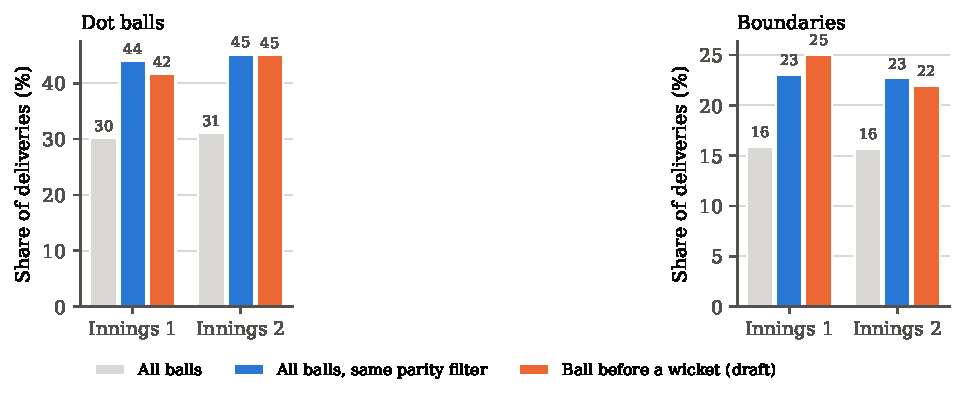
\includegraphics[width=\textwidth]{fig1_replication.pdf}
\caption{Dot balls and boundaries before wickets, with and without a like-for-like baseline. IPL 2008--2017. Grey bars show all deliveries; blue bars show all deliveries passing the draft's parity filter; orange bars show the delivery preceding a wicket as selected by the draft.}\label{fig:replication}
\end{figure}

Panel~B asks the forward-looking question directly: given the outcome of the striker's own previous ball, how likely is the striker to be dismissed on this one? Without any controls, dismissal is \emph{less} likely after a dot (\HazDotOne\% and \HazDotTwo\% in the two innings) than after 1--3 runs (\HazRunOne\% and \HazRunTwo\%). It is more likely after a six (\HazSixOne\% and \HazSixTwo\%). Section~\ref{sec:strategy} shows that the six result is also an artefact, this time of the stage of the innings.

% =====================================================================
\section{Empirical strategy}\label{sec:strategy}
% =====================================================================

\subsection{Specification}

We estimate linear probability models of the form
\begin{equation}\label{eq:main}
100 \cdot Y_{it} = \beta_D D_{i,t-1} + \beta_F F_{i,t-1} + \beta_S S_{i,t-1} + \mathbf{x}_{it}'\boldsymbol\gamma + \alpha_{b(i)} + \delta_{w(it)} + \nu_{v(it)} + \varepsilon_{it},
\end{equation}
where the omitted category is a previous ball yielding 1--3 runs, so that each $\beta$ is measured in percentage points relative to that category. The vector $\mathbf{x}_{it}$ contains a full set of indicators for the over interacted with the innings, the number of wickets lost (0--9), the striker's balls faced so far (13 bins), the striker's runs so far (9 bins) and the season. We refer to these as \emph{match-state fixed effects}. The terms $\alpha_{b}$, $\delta_{w}$ and $\nu_{v}$ are batter, bowler and venue fixed effects. Standard errors are clustered by match, which allows arbitrary correlation among all deliveries in a match. Linear probability models give coefficients on the scale of interest and accommodate high-dimensional fixed effects \citep{angrist2009mostly}. We estimate them with the alternating-projections method of \citet{berge2018fixest} and report logit average marginal effects as a robustness check. To test the innings and chase hypotheses we interact the three treatment indicators with an indicator for the second innings, or with an indicator that the required run rate is at least nine runs per over.

\subsection{Threats to identification}

\paragraph{Match state.} Figure~\ref{fig:over} shows why controls are essential. The dismissal rate per ball roughly triples between the middle overs and the 20th over, as batters trade wickets for runs. Over the same range the share of deliveries preceded by a six more than doubles and the share preceded by a dot halves. Any raw comparison therefore credits sixes with risk that belongs to the death overs, and credits dots with the safety of the early overs. Wickets lost, the striker's balls faced and runs scored matter in the same way: new batters are dismissed more often and play more dots.

\begin{figure}[tbp]
\centering
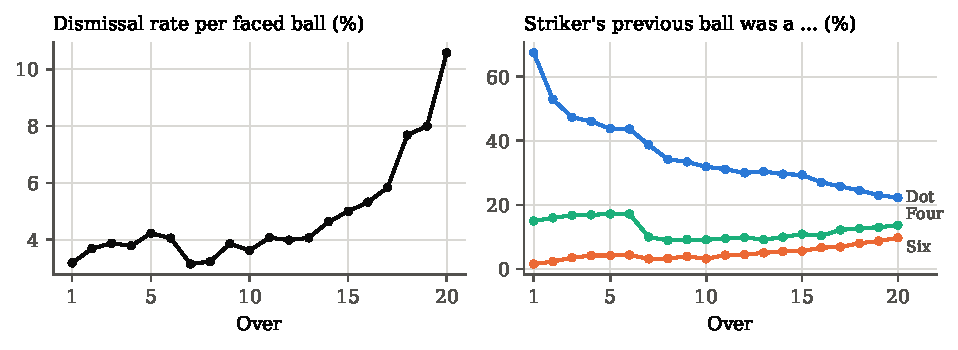
\includegraphics[width=\textwidth]{fig2_over_gradient.pdf}
\caption{The over gradient in dismissal risk and in the previous ball's outcome. Left: share of faced deliveries on which the striker is dismissed (bowler-credited). Right: share of faced deliveries whose striker's previous ball was a dot, a four or a six. IPL \Seasons.}\label{fig:over}
\end{figure}

\paragraph{Player quality and conditions.} Better batters hit more boundaries and are dismissed less often, and better bowlers concede more dots and take more wickets. The batter and bowler fixed effects absorb permanent differences in ability. In robustness checks we let both vary by season, and add team-innings and bowler-by-match (spell) fixed effects to absorb conditions on the day.

\paragraph{Selection on survival.} Only batters who survive to ball $t$ contribute an observation at $t$. We condition on balls faced and runs scored, so comparisons are always among batters at the same point in their innings with the same output. Within that set, the previous ball's outcome is what varies.

\paragraph{Small-group fixed effects.} Fixed effects for small groups of consecutive deliveries, such as an over, a bowler's spell or a batter's innings, induce a mechanical correlation between the lagged treatment and the demeaned outcome \citep{nickell1981biases}. This is the regression analogue of the streak-selection bias identified by \citet{miller2018surprised}. Dismissal ends a batter's sequence, so the bias is acute for the dismissal outcome. We therefore use such fixed effects only in robustness checks, and for the behavioural outcomes we estimate and remove the bias by permutation (Section~\ref{sec:behaviour}).

\paragraph{Inference.} With three treatment coefficients, two innings interactions per coefficient and several outcomes, some nominally significant estimates are expected by chance. We report Benjamini--Hochberg adjusted $p$-values for the six innings-specific tests \citep{benjamini1995controlling}. A null result is informative only if the estimates are precise, so we also report two one-sided tests of equivalence \citep{schuirmann1987comparison,lakens2017equivalence} against a smallest effect of interest of $\pm 10\%$ of the base dismissal rate ($\pm\EqDelta$\pp{}), together with minimum detectable effects.

% =====================================================================
\section{Results: dismissal}\label{sec:results}
% =====================================================================

\subsection{Main estimates}

Table~\ref{tab:main} reports estimates of equation~\eqref{eq:main}. Column~(1), without controls, reproduces the pattern of Panel~B of Table~\ref{tab:replication}: dismissal is \RawDot\pp{} less likely after a dot and \RawSix\pp{} more likely after a six. Adding the match-state fixed effects in column~(2) removes both. The dot coefficient becomes \StateDot\pp{} ($p=\StateDotP$) and the six coefficient \StateSix\pp{} ($p=\StateSixP$). Batter, bowler and venue fixed effects in column~(3) make little further difference. The dot coefficient is \FullDot\pp{} (95\% CI [\FullDotLo, \FullDotHi]), the six coefficient \FullSix\pp{} (95\% CI [\FullSixLo, \FullSixHi]) and the four coefficient \FullFour\pp{} (95\% CI [\FullFourLo, \FullFourHi]). The four coefficient is negative, the opposite sign to H2. The six and four coefficients are not significantly different from each other ($p=\SixMinusFourP$). Figure~\ref{fig:coefs} shows how the estimates move as controls are added.

\begin{table}[tbp]
\centering
\begin{threeparttable}
\caption{Dismissal and the striker's previous ball}\label{tab:main}
\small
\begin{tabular}{lcccccc}
\toprule
 & (1) & (2) & (3) & (4) & (5) & (6) \\
\midrule
Previous ball: dot & $-$0.43*** & 0.15 & 0.05 & 0.00 & 0.16 & $-$0.24 \\
 & (0.11) & (0.13) & (0.13) & (0.18) & (0.28) & (0.39) \\
\quad $\times$ second innings &  &  &  & 0.09 & $-$0.03 & 0.04 \\
 &  &  &  & (0.25) & (0.40) & (0.54) \\
Previous ball: four & $-$0.32* & $-$0.33* & $-$0.37** & $-$0.10 & 0.04 & $-$0.33 \\
 & (0.17) & (0.17) & (0.17) & (0.24) & (0.33) & (0.43) \\
\quad $\times$ second innings &  &  &  & $-$0.57* & $-$0.92** & $-$0.88 \\
 &  &  &  & (0.34) & (0.46) & (0.58) \\
Previous ball: six & 0.85*** & 0.12 & $-$0.04 & $-$0.08 & $-$0.06 & $-$0.40 \\
 & (0.28) & (0.29) & (0.29) & (0.38) & (0.45) & (0.52) \\
\quad $\times$ second innings &  &  &  & 0.09 & $-$0.13 & $-$0.07 \\
 &  &  &  & (0.54) & (0.66) & (0.73) \\
\midrule
Sample & All & All & All & All & Consecutive & Same over \\
Match-state FE &  & \checkmark & \checkmark & \checkmark & \checkmark & \checkmark \\
Batter, bowler, venue FE &  &  & \checkmark & \checkmark & \checkmark & \checkmark \\
Mean of outcome (pp) & 4.65 & 4.65 & 4.65 & 4.65 & 4.61 & 4.63 \\
Observations & 149,238 & 149,238 & 149,214 & 149,214 & 83,683 & 73,232 \\
\bottomrule
\end{tabular}

\begin{tablenotes}[flushleft]\footnotesize
\item \emph{Notes:} Linear probability models. The dependent variable is 100 if the striker is dismissed on the delivery by a bowler-credited mode (caught, bowled, lbw, stumped, hit wicket), 0 otherwise. The omitted category is a previous ball yielding 1--3 runs off the bat. Match-state FE are over$\times$innings, wickets lost, striker's balls faced (13 bins), striker's runs (9 bins) and season. ``Consecutive'' keeps deliveries whose striker also faced the immediately preceding delivery of the innings; ``Same over'' additionally requires the two to fall in the same over. Standard errors clustered by match in parentheses. *** $p<0.01$, ** $p<0.05$, * $p<0.1$.
\end{tablenotes}
\end{threeparttable}
\end{table}

\begin{figure}[tbp]
\centering
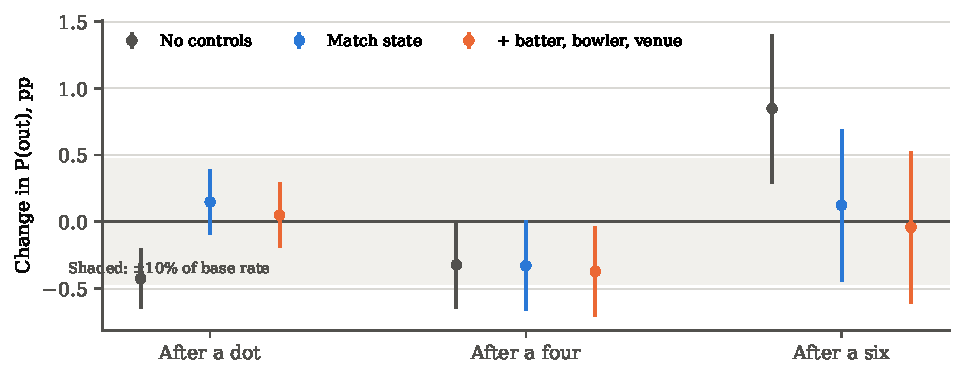
\includegraphics[width=\textwidth]{fig3_dismissal_coefs.pdf}
\caption{Change in the probability of dismissal after a dot, a four or a six, relative to a previous ball of 1--3 runs, as controls are added. Points are estimates of equation~\eqref{eq:main}; bars are 95\% confidence intervals clustered by match. The shaded band marks $\pm 10\%$ of the base dismissal rate.}\label{fig:coefs}
\end{figure}

These are precise nulls. The upper end of the 90\% confidence interval for the dot coefficient is \EqDotHi\pp{}, \EqDotRelHi\% of the base rate. A one-sided test rejects an increase of 10\% or more ($p=\EqDotPUp$). For a six the corresponding bound is \EqSixHi\pp{} (\EqSixRelHi\% of the base rate; $p=\EqSixPUp$). With the observed standard errors, the design has 80\% power to detect an effect of \MDEDot\pp{} after a dot (\MDEDotRel\% of the base rate) and \MDESix\pp{} after a six (\MDESixRel\%). Effects of the size implied by the folk theory, in which a dot or a boundary is a meaningful precursor to a wicket, would have been detected.

\subsection{Innings and chase pressure}

Columns~(4)--(6) of Table~\ref{tab:main} interact the treatments with the second innings. The pressure hypothesis predicts a positive dot$\times$second-innings interaction. The estimate is \IntDotX\pp{} ($p=\IntDotXP$). The overconfidence hypothesis predicts negative interactions for fours and sixes. The four interaction is \IntFourX\pp{} ($p=\IntFourXP$), the largest estimate in a predicted direction, and the six interaction is \IntSixX\pp{} ($p=\IntSixXP$). After a Benjamini--Hochberg correction across the six innings-specific coefficients, the smallest adjusted $p$-value is \BHMinP. Restricting the sample to consecutive deliveries (column~5) makes the four interaction significant at the 5\% level. The restriction to the same over (column~6) does not, and no corresponding pattern appears for sixes, which should carry the stronger overconfidence signal. The dot interaction is close to zero in every column.

The second-innings indicator is a blunt proxy for pressure, since many chases are comfortable. Table~\ref{tab:chase} uses the required run rate instead. Restricting to \ChaseN{} deliveries in chases with a known target, we interact the treatments with an indicator that the required rate is at least nine runs per over (\ChaseHighShare\% of chase deliveries). The regression also includes fixed effects for bins of the required rate. If dot balls build pressure, they should do so most in a demanding chase. Instead the dot$\times$high-RRR interaction is \ChaseDotHi\pp{} ($p=\ChaseDotHiP$). The only interaction significant at the 10\% level is for sixes (\ChaseSixHi\pp{}, $p=\ChaseSixHiP$), and its sign is the reverse of the overconfidence hypothesis, which places overconfidence in the unconstrained first innings.

\begin{table}[tbp]
\centering
\begin{threeparttable}
\caption{Chase pressure: interactions with the required run rate}\label{tab:chase}
\small
\begin{tabular}{lc}
\toprule
 & Chases \\
\midrule
Previous ball: dot & 0.27 \\
 & (0.21) \\
Dot $\times$ RRR $\geq 9$ & -0.38 \\
 & (0.30) \\
Previous ball: four & -0.54* \\
 & (0.30) \\
Four $\times$ RRR $\geq 9$ & -0.21 \\
 & (0.47) \\
Previous ball: six & -0.80 \\
 & (0.50) \\
Six $\times$ RRR $\geq 9$ & 1.42* \\
 & (0.79) \\
\midrule
Match-state, RRR-bin FE & \checkmark \\
Batter, bowler, venue FE & \checkmark \\
Mean of outcome (pp) & 4.68 \\
Observations & 70,656 \\
\bottomrule
\end{tabular}

\begin{tablenotes}[flushleft]\footnotesize
\item \emph{Notes:} Second-innings deliveries in matches with a known target (Duckworth--Lewis matches excluded) and runs still required. RRR is the required run rate before the delivery. Controls as in column~(3) of Table~\ref{tab:main}, plus RRR-bin fixed effects (<6, 6--8, 8--10, 10--12, 12+). Standard errors clustered by match. *** $p<0.01$, ** $p<0.05$, * $p<0.1$.
\end{tablenotes}
\end{threeparttable}
\end{table}

\subsection{Runs of dots}

Pressure is often described as cumulative: one dot is routine, but three in a row are not. Figure~\ref{fig:dotrun} (left panel) replaces the single dot indicator with indicators for the length of the run of consecutive dots ending at the previous ball (1, 2, 3, 4 or more). No dose response appears. Each coefficient is small and statistically indistinguishable from zero, and the point estimates for three or more dots are negative. The right panel shows the corresponding estimates for the probability of a boundary, discussed in Section~\ref{sec:behaviour}.

\begin{figure}[tbp]
\centering
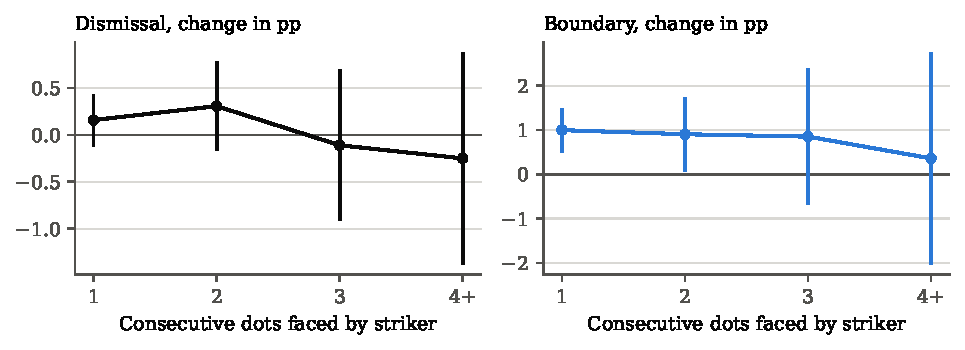
\includegraphics[width=\textwidth]{fig5_dot_runs.pdf}
\caption{Runs of consecutive dot balls. Each point is the change in the outcome on the current ball (percentage points) when the striker's previous ball ended a run of $k$ dots, relative to a previous ball of 1--3 runs, with controls as in column~(3) of Table~\ref{tab:main}. Bars are 95\% confidence intervals clustered by match.}\label{fig:dotrun}
\end{figure}

% =====================================================================
\section{Robustness}\label{sec:robust}
% =====================================================================

Table~\ref{tab:robust} re-estimates column~(3) of Table~\ref{tab:main} under \RobRows{} alternative choices. Across all of them, the dot coefficient ranges from \RobDotMin{} to \RobDotMax\pp{} and the six coefficient from \RobSixMin{} to \RobSixMax\pp.

\begin{table}[tbp]
\centering
\begin{threeparttable}
\caption{Robustness of the dismissal estimates}\label{tab:robust}
\footnotesize
\setlength{\tabcolsep}{4pt}
\begin{tabular}{lccccc}
\toprule
 & Dot & Four & Six & Mean (pp) & N \\
\midrule
Baseline & 0.05 (0.13) & $-$0.37** (0.17) & $-$0.04 (0.29) & 4.65 & 149,214 \\
Outcome includes run outs & 0.10 (0.13) & $-$0.38** (0.18) & 0.02 (0.30) & 4.91 & 149,214 \\
Outcome: caught only & 0.13 (0.11) & $-$0.38** (0.15) & $-$0.07 (0.25) & 3.25 & 149,214 \\
Outcome: bowled or lbw only & $-$0.12* (0.07) & $-$0.04 (0.09) & $-$0.06 (0.15) & 1.24 & 149,214 \\
Strict dot (no extras) & 0.08 (0.13) & $-$0.37** (0.17) & $-$0.04 (0.29) & 4.65 & 149,214 \\
Previous ball of the innings (any striker) & 0.02 (0.12) & $-$0.41** (0.17) & $-$0.27 (0.28) & 4.59 & 158,256 \\
Seasons 2008--2017 (draft sample) & 0.11 (0.13) & $-$0.32* (0.18) & $-$0.01 (0.31) & 4.64 & 136,270 \\
Season 2018 only (held out) & $-$0.44 (0.39) & $-$0.92* (0.53) & $-$0.34 (0.79) & 4.80 & 12,946 \\
Striker has faced 5+ balls & 0.12 (0.15) & $-$0.28 (0.20) & $-$0.20 (0.30) & 4.84 & 113,861 \\
Top order (0--5 wickets down) & 0.06 (0.13) & $-$0.37** (0.17) & $-$0.05 (0.30) & 4.36 & 137,014 \\
Excluding death overs (16--20) & 0.13 (0.13) & $-$0.41** (0.18) & $-$0.03 (0.34) & 3.90 & 116,081 \\
Team-innings FE & 0.19 (0.13) & $-$0.17 (0.17) & $-$0.02 (0.29) & 4.65 & 149,214 \\
Bowler-by-match FE (the spell) & 0.28** (0.13) & $-$0.04 (0.18) & 0.20 (0.29) & 4.65 & 149,205 \\
Batter-season and bowler-season FE & 0.05 (0.13) & $-$0.33* (0.17) & $-$0.05 (0.29) & 4.65 & 149,166 \\
Two-way clustering (match, batter) & 0.05 (0.12) & $-$0.37** (0.18) & $-$0.04 (0.34) & 4.65 & 149,214 \\
\bottomrule
\end{tabular}

\begin{tablenotes}[flushleft]\footnotesize
\item \emph{Notes:} Each row reports the coefficients on a previous dot, four and six (percentage points; omitted category 1--3 runs) from a separate regression. Unless stated, controls are match-state, batter, bowler and venue fixed effects, and standard errors (in parentheses) are clustered by match. ``Strict dot'' requires no extras on the previous ball and adds an indicator for byes and leg byes. ``Previous ball of the innings'' uses the immediately preceding faced delivery whoever faced it, the definition closest to the earlier draft, and adds an indicator for a wicket on that ball. The 2018 season uses state fixed effects only. *** $p<0.01$, ** $p<0.05$, * $p<0.1$.
\end{tablenotes}
\end{threeparttable}
\end{table}

\paragraph{Outcome definitions.} Counting run outs as dismissals, or restricting to caught dismissals (the mode most associated with an ambitious shot), leaves the estimates unchanged. Restricted to bowled and lbw dismissals, the dot coefficient is slightly negative.

\paragraph{Treatment definitions.} Defining a dot strictly, with no runs of any kind, makes no difference. Using the previous delivery of the innings whoever faced it, the team-level notion of pressure closest to the earlier draft, also produces null results for dots and sixes.

\paragraph{Samples.} The estimates are similar on the draft's 2008--2017 sample and in the held-out 2018 season, although the 2018 estimates are imprecise. They are also similar for strikers who have faced at least five balls, which removes the most fragile phase of an innings, for innings with at most five wickets down, and outside the death overs.

\paragraph{Controls.} Batter-season and bowler-season fixed effects allow ability to change over time, and leave the results unchanged. Team-innings fixed effects absorb pitch and weather on the day. Bowler-by-match fixed effects absorb a bowler's form within a spell. With these, the dot coefficient rises to \RobDotMax\pp{}, the one estimate in the table that is positive and significant at 5\%. Two considerations argue against reading this as evidence for H1. First, a spell contains about two dozen deliveries and few dismissals, which is exactly the small-group setting in which demeaning a lagged indicator against an outcome that ends a batter's sequence produces bias of the kind discussed in Section~\ref{sec:strategy}. Second, even this estimate is below the 10\% equivalence margin in its point value, and it is one of \RobRows{} specifications.

\paragraph{Functional form and inference.} A logit model with the match-state controls gives average marginal effects of \LogitDot\pp{} for a dot ($p=\LogitDotP$), \LogitFour\pp{} for a four ($p=\LogitFourP$) and \LogitSix\pp{} for a six ($p=\LogitSixP$). Two-way clustering by match and batter \citep{cameron2011robust} leaves the inference unchanged.

% =====================================================================
\section{The behavioural response}\label{sec:behaviour}
% =====================================================================

The previous ball does not predict dismissal. Does it predict anything? Table~\ref{tab:behaviour} replaces the dismissal outcome with the striker's scoring on the current ball, using the controls of column~(3) of Table~\ref{tab:main}. Figure~\ref{fig:behaviour} expresses the estimates relative to each outcome's mean.

\begin{table}[tbp]
\centering
\begin{threeparttable}
\caption{What the striker does next}\label{tab:behaviour}
\small
\begin{tabular}{lccccc}
\toprule
 & Boundary & Six & Dot & Runs & Out \\
\midrule
Previous ball: dot & 0.76*** & 0.19 & -0.54* & 0.03*** & 0.05 \\
 & (0.25) & (0.14) & (0.30) & (0.01) & (0.13) \\
Previous ball: four & -0.38 & 0.01 & 0.48 & -0.01 & -0.37** \\
 & (0.32) & (0.19) & (0.38) & (0.01) & (0.17) \\
Previous ball: six & 2.35*** & 1.25*** & -1.48*** & 0.12*** & -0.04 \\
 & (0.53) & (0.35) & (0.56) & (0.02) & (0.29) \\
\midrule
Units & pp & pp & pp & runs & pp \\
Match-state FE & \checkmark & \checkmark & \checkmark & \checkmark & \checkmark \\
Batter, bowler, venue FE & \checkmark & \checkmark & \checkmark & \checkmark & \checkmark \\
Mean of outcome & 16.91 & 4.89 & 32.45 & 1.308 & 4.65 \\
Observations & 149,214 & 149,214 & 149,214 & 149,214 & 149,214 \\
\bottomrule
\end{tabular}

\begin{tablenotes}[flushleft]\footnotesize
\item \emph{Notes:} Each column is a separate linear probability model (column ``Runs'': OLS on runs off the bat). Outcomes refer to the current delivery: a boundary (4 or 6 off the bat), a six, a dot (no runs off the bat and no dismissal), runs off the bat, and a bowler-credited dismissal. The omitted category is a previous ball yielding 1--3 runs. Controls as in column~(3) of Table~\ref{tab:main}. Standard errors clustered by match. *** $p<0.01$, ** $p<0.05$, * $p<0.1$.
\end{tablenotes}
\end{threeparttable}
\end{table}

\begin{figure}[tbp]
\centering
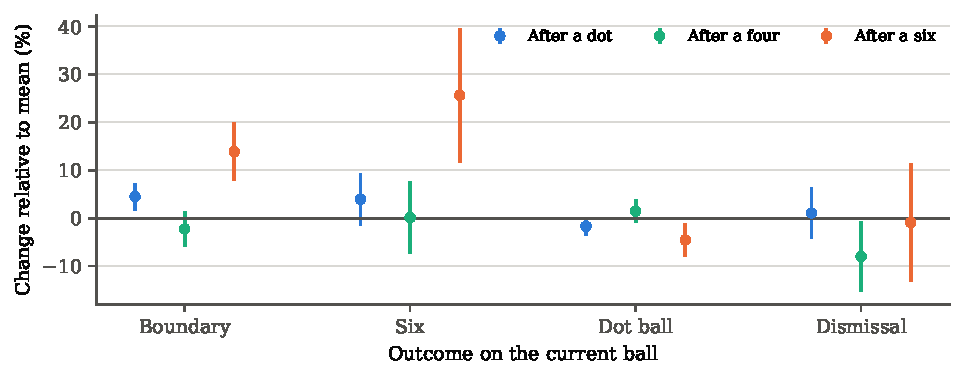
\includegraphics[width=\textwidth]{fig4_behaviour.pdf}
\caption{Outcomes on the current ball by the striker's previous ball, relative to a previous ball of 1--3 runs, as a percentage of each outcome's mean. Bars are 95\% confidence intervals clustered by match.}\label{fig:behaviour}
\end{figure}

Two patterns stand out. After a dot, the striker is \MBoundaryDot\pp{} more likely to hit a boundary ($p=\MBoundaryDotP$), \MBoundaryDotRel\% of the mean, and less likely to play another dot. The left panel of Figure~\ref{fig:dotrun} showed no rise in dismissals after runs of dots. The right panel shows that the boundary response is present after one or two dots. After a six, the striker is \MBoundarySix\pp{} more likely to hit another boundary ($p=\MBoundarySixP$, \MBoundarySixRel\% of the mean) and \MSixSix\pp{} more likely to hit another six ($p=\MSixSixP$, \MSixSixRel\% of the mean). Expected runs off the bat rise by \MRunsSix{} after a six and by \MRunsDot{} after a dot. Neither response is accompanied by a detectable change in dismissal risk. Fours, unlike sixes, are not followed by more boundaries.

\subsection{Order or conditions?}

A positive association between consecutive boundaries need not reflect any response to the previous ball. A batter facing a weak bowler on a flat pitch will hit many boundaries, so any ball that follows a boundary is more likely to come from such an innings. The batter, bowler and venue fixed effects absorb permanent differences, but not conditions on the day. Table~\ref{tab:fe} adds progressively tighter fixed effects: match, team innings, bowler by match and, most demanding, batter by innings. The last compares deliveries within the same batter's innings.

\begin{table}[tbp]
\centering
\begin{threeparttable}
\caption{Boundary on the current ball: tightening the fixed effects}\label{tab:fe}
\footnotesize
\setlength{\tabcolsep}{4pt}
\begin{tabular}{lccccc}
\toprule
 & (1) & (2) & (3) & (4) & (5) \\
\midrule
Previous ball: dot & 0.76*** & 0.79*** & 0.66*** & 0.72*** & 0.18 \\
 & (0.25) & (0.25) & (0.25) & (0.25) & (0.25) \\
Previous ball: four & $-$0.38 & $-$0.62* & $-$0.90*** & $-$4.32*** & $-$3.07*** \\
 & (0.32) & (0.32) & (0.32) & (0.32) & (0.33) \\
Previous ball: six & 2.35*** & 2.00*** & 1.90*** & $-$1.99*** & 1.00* \\
 & (0.53) & (0.53) & (0.53) & (0.53) & (0.54) \\
\midrule
Match-state FE & \checkmark & \checkmark & \checkmark & \checkmark & \checkmark \\
Batter FE & \checkmark & \checkmark & \checkmark & \checkmark &  \\
Bowler FE & \checkmark & \checkmark & \checkmark &  & \checkmark \\
Match FE &  & \checkmark &  &  &  \\
Team-innings FE &  &  & \checkmark &  &  \\
Bowler-by-match FE &  &  &  & \checkmark &  \\
Batter-by-innings FE &  &  &  &  & \checkmark \\
Observations & 149,214 & 149,214 & 149,214 & 149,205 & 148,624 \\
\bottomrule
\end{tabular}

\begin{tablenotes}[flushleft]\footnotesize
\item \emph{Notes:} Dependent variable is 100 if the current delivery is hit for four or six. Column~(1) uses the controls of column~(3) of Table~\ref{tab:main}. Columns~(2)--(5) add or substitute the fixed effects named. Standard errors clustered by match. These estimates are not corrected for the finite-sequence bias; see Table~\ref{tab:perm}. *** $p<0.01$, ** $p<0.05$, * $p<0.1$.
\end{tablenotes}
\end{threeparttable}
\end{table}

The uncorrected estimates in columns~(4) and~(5) change sharply, and the four and six coefficients turn negative. That is what the finite-sequence bias predicts. Within a short group of deliveries, a ball that follows a boundary is a ball that is not itself the boundary, so demeaning within the group pushes the coefficient on a lagged boundary downward \citep{nickell1981biases,miller2018surprised}. To measure this bias and the role of conditions on the day, we use a permutation test \citep{young2019channeling}. Within each of the \BatterInnings{} batter-innings (on average \BatterInningsMeanBalls{} faced balls), we randomly reorder the striker's runs across deliveries. The dismissal ball stays in place, and the match state, opponents and balls-faced counts stay attached to their positions. Runs scored so far are recomputed for each permutation. A permuted dataset has the same batter-innings, the same composition of each innings and the same conditions on the day as the real data. Only the order of balls within an innings is random. Re-estimating each specification on \PermR{} permuted datasets gives the distribution of each coefficient under the null that order carries no information. The mean of that distribution captures the composition and finite-sequence effects. The difference between the observed coefficient and the null mean is the order effect.

\begin{table}[tbp]
\centering
\begin{threeparttable}
\caption{Order effects net of the permutation null}\label{tab:perm}
\footnotesize
\setlength{\tabcolsep}{4pt}
\begin{tabular}{lccccccccc}
\toprule
 & \multicolumn{3}{c}{Previous ball: dot} & \multicolumn{3}{c}{Previous ball: four} & \multicolumn{3}{c}{Previous ball: six} \\
\cmidrule(lr){2-4}\cmidrule(lr){5-7}\cmidrule(lr){8-10}
Fixed effects & Est. & Null & Corr. & Est. & Null & Corr. & Est. & Null & Corr. \\
\midrule
Baseline & 0.76 & $-$0.16 & 0.92*** & $-$0.38 & $-$0.33 & $-$0.05 & 2.35 & 0.54 & 1.81*** \\
Match & 0.79 & $-$0.13 & 0.92*** & $-$0.62 & $-$0.56 & $-$0.06 & 2.00 & 0.24 & 1.76*** \\
Team innings & 0.66 & $-$0.20 & 0.86*** & $-$0.90 & $-$0.82 & $-$0.08 & 1.90 & 0.07 & 1.83*** \\
Bowler by match & 0.72 & $-$0.22 & 0.94*** & $-$4.32 & $-$3.58 & $-$0.74** & $-$1.99 & $-$2.63 & 0.64 \\
Batter by innings & 0.18 & $-$1.15 & 1.33*** & $-$3.07 & $-$3.53 & 0.46 & 1.00 & $-$1.19 & 2.19*** \\
\bottomrule
\end{tabular}

\begin{tablenotes}[flushleft]\footnotesize
\item \emph{Notes:} ``Est.'' is the observed coefficient from Table~\ref{tab:fe}. ``Null'' is the mean coefficient across \PermR{} datasets in which each striker's runs are randomly reordered within the innings, holding the dismissal ball, match state and opponents fixed. ``Corr.'' is the difference. Stars give two-sided permutation $p$-values for the difference: *** $p<0.01$, ** $p<0.05$, * $p<0.1$.
\end{tablenotes}
\end{threeparttable}
\end{table}

Table~\ref{tab:perm} and Figure~\ref{fig:perm} report the results. The null means for the batter-innings specification are large and negative, which confirms the size of the finite-sequence bias. Against these benchmarks the observed coefficients are clearly unusual. In the batter-innings specification the corrected after-dot effect is \PEDotCorr\pp{} ($p=\PEDotP$) and the corrected after-six effect is \PESixCorr\pp{} ($p=\PESixP$). In the pooled specification the corresponding figures are \PADotCorr\pp{} ($p=\PADotP$) and \PASixCorr\pp{} ($p=\PASixP$). Across all five specifications the corrected after-six effect lies between \PDSixCorr{} and \PESixCorr\pp{}. The corrected after-four effect is small throughout. The ordering of balls within a batter's innings therefore carries information beyond the conditions that the innings shares.

\begin{figure}[tbp]
\centering
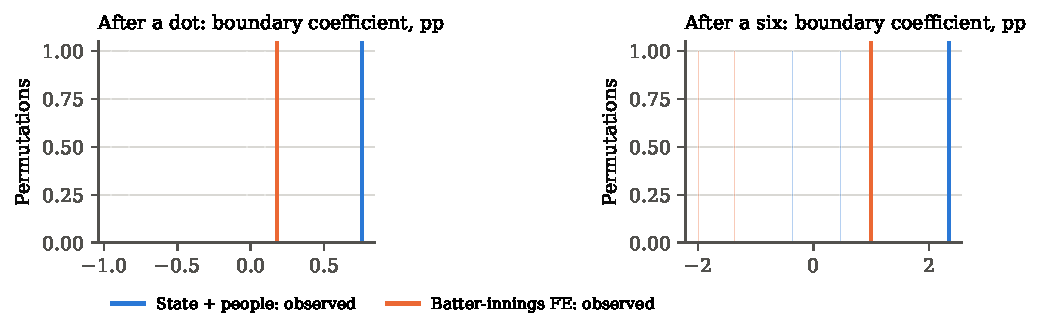
\includegraphics[width=\textwidth]{fig6_permutation.pdf}
\caption{Permutation distributions of the boundary coefficients. Histograms show coefficients across \PermR{} datasets in which each striker's runs are randomly reordered within the innings. Vertical lines mark the observed coefficients. Blue: match-state, batter, bowler and venue fixed effects. Orange: batter-innings fixed effects.}\label{fig:perm}
\end{figure}

\subsection{Robustness of the behavioural response}

Table~\ref{tab:momrobust} re-estimates the boundary equation on alternative samples and with season-varying player effects. The after-dot coefficient ranges from \RbDotMin{} to \RbDotMax\pp{} and the after-six coefficient from \RbSixMin{} to \RbSixMax\pp{}. Both are present in each innings, outside the death overs, for set batters, and when the previous ball was bowled in the same over by the same bowler. In the single held-out season of 2018 the point estimates are at least as large, although the after-dot estimate is imprecise. In chases the after-dot boundary response does not grow with the required run rate (interaction \HetDotHi\pp{}, $p=\HetDotHiP$). The response therefore appears to be a general feature of how batters manage an innings, not a reaction to the scoreboard.

\begin{table}[tbp]
\centering
\begin{threeparttable}
\caption{Robustness of the boundary response}\label{tab:momrobust}
\footnotesize
\setlength{\tabcolsep}{4pt}
\begin{tabular}{lccccc}
\toprule
 & Dot & Four & Six & Mean (pp) & N \\
\midrule
Baseline & 0.76*** (0.25) & $-$0.38 (0.32) & 2.35*** (0.53) & 16.91 & 149,214 \\
Seasons 2008--2017 & 0.73*** (0.25) & $-$0.34 (0.33) & 2.20*** (0.56) & 16.71 & 136,270 \\
Season 2018 only & 1.43 (0.94) & $-$0.32 (1.10) & 4.11*** (1.52) & 18.99 & 12,946 \\
Consecutive balls only & 1.05*** (0.36) & $-$0.33 (0.43) & 2.53*** (0.63) & 17.49 & 83,683 \\
Same over only & 0.81* (0.47) & $-$0.68 (0.51) & 2.13*** (0.69) & 17.71 & 73,232 \\
Striker has faced 5+ balls & 0.67** (0.27) & $-$0.42 (0.35) & 2.23*** (0.56) & 18.03 & 113,861 \\
Excluding death overs & 0.61** (0.26) & $-$0.82** (0.35) & 3.33*** (0.65) & 16.00 & 116,081 \\
First innings & 0.75** (0.33) & $-$0.81* (0.44) & 1.74** (0.74) & 16.99 & 77,512 \\
Second innings & 0.80** (0.35) & $-$0.53 (0.46) & 2.40*** (0.77) & 16.82 & 71,689 \\
Batter-season, bowler-season FE & 0.67*** (0.25) & $-$1.23*** (0.32) & 1.40*** (0.53) & 16.91 & 149,166 \\
\bottomrule
\end{tabular}

\begin{tablenotes}[flushleft]\footnotesize
\item \emph{Notes:} Dependent variable is 100 if the current delivery is hit for four or six. Each row is a separate regression with the controls of column~(3) of Table~\ref{tab:main} unless stated. Standard errors clustered by match in parentheses. *** $p<0.01$, ** $p<0.05$, * $p<0.1$.
\end{tablenotes}
\end{threeparttable}
\end{table}

% =====================================================================
\section{Discussion}\label{sec:discussion}
% =====================================================================

\paragraph{Interpretation.} The evidence fits a simple account. After a dot, batters score more aggressively, probably to restore the run rate and rotate the strike. After a six, they continue to attack, perhaps because the six revealed something about the bowler, the length or the field that makes another attacking shot attractive. Neither adjustment raises the probability of dismissal. This is what we would expect if batters choose shots so that the extra reward is not bought with extra risk, or if bowlers respond in ways that offset the batter's adjustment. The data cannot separate these explanations, because ball-by-ball records do not include the delivery's line and length, the shot attempted or the field set. The second explanation parallels the equilibrium adjustment documented by \citet{green2018hot}. Either way, the folk theory fails on the specific point at issue. Neither the pressure of a dot ball nor the exhilaration of a boundary shows up as an increased chance of getting out.

\paragraph{Why the belief persists.} The belief is easy to form from memorable cases. A wicket that follows a boundary or a run of dots makes a vivid story, and observers recall it more easily than the many boundaries and dots that are followed by nothing \citep{tversky1973availability}. The draft that preceded this paper fell into a statistical version of the same trap: it compared the ball before each wicket with a baseline that had been selected differently. The prospective question, how often a dot is followed by a wicket compared with a single, is the one that the hypothesis concerns, and its answer is ``no more often''.

\paragraph{Practical implications.} For bowling sides the results caution against strategies that rely on a batter's supposed loss of composure after a boundary or a run of dots. For batting sides they suggest that the aggressive response to a dot ball, which coaches often discourage, carries no detectable cost in wickets. For modellers, dismissal can be treated as independent of the previous ball given the match state, but boundary probabilities cannot. Simulators that ignore short-run dependence in scoring will understate the variance of team totals.

\paragraph{Limitations.} The sample covers one competition, eleven seasons and one format. In longer formats a dot ball carries less scoreboard cost, so the pressure it creates, and batters' responses to it, may differ. The data record outcomes, not intentions. We observe neither the shot attempted, nor the field, nor the bowler's line and length. We cannot therefore tell whether batters attempt more aggressive shots after a dot or simply find them more often. The equivalence margins rule out effects larger than about a tenth of the base rate, but cannot exclude smaller ones. Finally, the permutation test treats the order of balls within an innings as exchangeable under the null. A smooth within-innings trend in aggression, beyond what balls faced, runs scored and over capture, could account for part of the order effect.

% =====================================================================
\section{Conclusion}\label{sec:conclusion}
% =====================================================================

Cricket's folk theory holds that dot balls build pressure and boundaries breed overconfidence, and that both lead to wickets. An earlier version of this study appeared to confirm it. Re-examined, the confirmation came from a selection artefact. With \FacedDeliveries{} deliveries from eleven IPL seasons, the outcome of a batter's previous ball does not predict dismissal once the match state is held fixed, and the estimates are precise enough to rule out effects larger than a tenth of the base rate. Batters do respond to the previous ball. They hit boundaries more often after a dot and after a six, and the permutation evidence shows that this response depends on the order of balls rather than on the day's conditions. The response comes without a detectable cost in wickets.

Two extensions would sharpen these conclusions. Ball-tracking and shot-type data would show whether batters change the shots they attempt or only how often those shots succeed. Data from Test and one-day cricket would show whether the same patterns hold when the scoreboard cost of a dot ball is lower.

\section*{Data availability statement}
The ball-by-ball data are the public IPL deliveries and matches files (2008--2018) originally distributed through Kaggle. A copy with SHA-256 checksums is included in the replication repository, together with code that reproduces every table, figure and number in the paper from the raw files with a single command (\texttt{make}).

\section*{Declaration of conflicting interests}
The author declares no potential conflicts of interest with respect to the research, authorship and/or publication of this article.

\section*{Funding}
The author received no financial support for the research, authorship and/or publication of this article.

\bibliographystyle{apalike}
\bibliography{references}

\appendix
\section{Data construction}\label{app:data}

\paragraph{Source and coverage.} The deliveries file contains one row per delivery, including wides and no-balls, with the over, the ball number within the over, the striker, non-striker and bowler, runs off the bat, extras by type, and the dismissed player and mode of dismissal. The matches file supplies the season, venue, result and an indicator for matches decided by the Duckworth--Lewis method. The draft that preceded this paper used the 2008--2017 seasons: \OrigDeliveries{} deliveries from \OrigMatches{} matches.

\paragraph{Ordering and duplicates.} Deliveries are ordered within each innings by their position in the file, which follows the scorer's sequence. Match 7946 (2018) contains \DroppedDuplicates{} rows that exactly duplicate earlier rows of the same innings, one of them recorded out of sequence. These are removed. Super-over rows (innings 3 and 4) are removed.

\paragraph{Faced deliveries.} A wide is not a ball faced and is dropped after the match state is computed. No-balls are balls faced and are retained. The striker's balls faced and runs scored before each delivery are cumulative counts within the batter's innings.

\paragraph{Previous ball.} The striker's previous ball is the last faced delivery by the same striker in the same innings. It is \emph{consecutive} if it was also the immediately preceding faced delivery of the innings (\ConsecutiveShare\% of the analysis sample). Previous-ball categories use runs off the bat: dot (0), 1--3 runs (1, 2, 3, and the rare 5 or 7), four (4) and six (6).

\paragraph{Dismissals.} Bowler-credited dismissals are caught, caught and bowled, bowled, lbw, stumped and hit wicket, and count only when the striker is the player dismissed. Run outs (\RunOuts{} in the raw data), retirements and obstructing the field are excluded from the main outcome.

\paragraph{Chase state.} The target is the first-innings total plus one. Runs required, balls remaining (120 minus legal balls bowled) and the required run rate are computed before each delivery for second innings not decided by the Duckworth--Lewis method.

\end{document}
